% !TEX root = ../CourseOT.tex

%%%%%%%%%%%%%%%%%%%%%%%%%%%%%%%%%%%%%%%%%%%%%%%%%%%%%%%%%%%%%%%%%%%%%%%%%%%
%%%%%%%%%%%%%%%%%%%%%%%%%%%%%%%%%%%%%%%%%%%%%%%%%%%%%%%%%%%%%%%%%%%%%%%%%%%
%%%%%%%%%%%%%%%%%%%%%%%%%%%%%%%%%%%%%%%%%%%%%%%%%%%%%%%%%%%%%%%%%%%%%%%%%%%
\section{Monge Problem between Measures}

%%%%%%%%%%%%%%%%%%%%%%%%%%%%%%%%%%%%%%%%%%%%%%%%%%%%%%%%%%%%%%%%%%%%%%%%%%%
\subsection{Measures}


%%%
\paragraph{Histograms}

We will interchangeably the term histogram or probability vector for any element $\a \in \simplex_n$ that belongs to the probability simplex
\eq{
	\simplex_n \eqdef \enscond{\a \in \RR_+^n}{ \sum_{i=1}^n \a_i = 1 }.
}


%%%
\paragraph{Discrete measure, empirical measure}


A discrete measure with weights $\a$ and locations $x_1,\dots,x_n\in\X$ reads
\eql{\label{eq-discr-meas}
	\al = \sum_{i=1}^n \a_i \de_{x_i}
}
where $\de_x$ is the Dirac at position $x$, intuitively a unit of mass which is infinitely concentrated at location $x$. Such as measure describes a probability measure if, additionally, $\a\in\simplex_n$, and more generally a positive measure if each of the ``weights'' described in vector $\a$ is positive itself. 

Lagrangian vs Eulerian. 


%%%%
\paragraph{Measures}


We denote $\Mm_+(\X)$ the set of all positive measures on $\X$. The set of probability measures is denoted $\Mm_+^1(\X)$, which means that any $\al \in \Mm_+^1(\X)$ is positive, and that $\al(\X)=\int_\Xx \d\al = 1$. 



%%%%
\paragraph{Radon measures}

To be make use of tools from convex analysis and optimization (and in particular duality), we assume a bit more on the measures, namely that they are Radon measures $\Mm(\X)$ on the space $\X$. This 
requires that $\X$ is equipped with a distance, usually denoted $\dist$, because one can only access a measure by ``testing'' (integrating) it against continuous functions, denoted $f \in \Cc(\X)$. 
%
Integration of $f \in \Cc(\X)$ against a discrete measure $\al$ computes a sum
\eq{ 
	\int_\X f(x) \d\al(x) = \sum_{i=1}^n \a_i f(x_i).
}

An arbitrary measure $\al \in \Mm(\X)$ (which needs not to have a density nor be a sum of Diracs) is defined by the fact that it can be integrated agains any continuous function $f \in \Cc(\X)$ and obtain $\int_\X f(x) \d\al(x) \in \RR$. If $\X$ is not compact, one should also impose that $f$ has compact support or at least as $0$ limit at infinity. 

Measure as thus in some sense ``less regular'' than functions, but more regular than distributions (which are dual to smooth functions). For instance, the derivative of a Dirac is not a measure.



%%%%%
\paragraph{Relative densities}

%TODO : ref measures
More general measures, for instance on $\X=\RR^\dims$ (where $\dims \in \NN^*$ is the dimension), can have a density $\d\al(x)=\density{\al}(x)\d x$ w.r.t. the Lebesgue measure, often denoted $\density{\al} = \frac{\d\al}{\d x}$, which means that 
\eq{
	\foralls h \in \Cc(\RR^\dims), \quad
	\int_{\RR^\dims} h(x) \d\al(x) =  \int_{\RR^\dims} h(x) \density{\al}(x) \d x.
}



%%%%%
\paragraph{Probabilistic interpretation}

Radon measures can also be viewed as representing the distributions of random variables. A random variable $X$ on $\X$ is actually a map $X : \Om \rightarrow \X$ from some abstract (often un-specified) probabized space $(\Om,\PP)$, and its distribution $\al$ is the Radon measure $X \in \Mm_+^1(\X)$ such that $\PP(X \in A) = \al(A)=\int_A \d\al(x)$.


%%%%%%%%%%%%%%%%%%%%%%%%%%%%%%%%%%%%%%%%%%%%%%%%%%%%%%%%%%%%%%%%%%%%%%%%%%%
\subsection{Push Forward}
  
  
For some continuous map $\T : \X \rightarrow \Y$, we define the pushforward operator $\T_\sharp : \Mm(X) \rightarrow \Mm(Y)$. 
%
For discrete measures~\eqref{eq-discr-meas}, the pushforward operation consists simply in moving the positions of all the points in the support of the measure
\eq{
	\T_{\sharp} \al \eqdef \sum_i \a_i \de_{\T(x_i)}.
}
For more general measures, for instance for those with a density, the notion of push-forward plays a fundamental to describe spatial modifications of probability measures. The formal definition reads as follow.

\begin{defn}[Push-forward]\label{defn-pushfwd}
For $\T : \X \rightarrow \Y$, the push forward measure $\be = \T_\sharp \al \in \Mm(\Y)$ of some $\al \in \Mm(\X)$ reads
\eql{\label{eq-push-fwd}
	\foralls h \in \Cc(\Y), \quad \int_\Y h(y) \d \be(y) = \int_\X h(\T(x)) \d\al(x).
	% = \int_X h(T(x)) \density{\al}(x) \d x %%%% y=T(x)   dy=|T'(x)| dx
	% = \int_Y h(y) \density{\al}(T^{-1}(y)) 1/|T'(x)| \d y 
	% = \int_Y h(y) \density{\be}(y) \d y
	%  \density{\al}(T^{-1}(y)) 1/|T'(x)| = \density{\be}(y)
}
Equivalently, for any measurable set $B \subset \Y$, one has
\eql{\label{eq-equiv-pushfwd}
	\be(B) = \al( \enscond{x \in \X}{\T(x) \in B} ).
}
Note that $\T_\sharp$ preserves positivity and total mass, so that if $\al \in \Mm_+^1(\X)$ then $\T_\sharp \al \in \Mm_+^1(\Y)$. 
\end{defn}

Intuitively, a measurable map $T: \X\rightarrow \Y$, can be interpreted as a function ``moving'' a single point from a measurable space to another. The more general extension $T_\sharp$ can now ``move'' an entire probability measure on $\X$ towards a new probability measure on $\Y$. The operator $T_\sharp$ ``pushes forward'' each elementary mass of a measure $\al$ on $\X$ by applying the map $T$ to obtain then an elementary mass in $\Y$, to build on aggregate a new measure on $\Y)$ written $T_{\sharp}\al$.  Note that such a push-forward $\T_\sharp : \Mm_+^1(\X) \rightarrow \Mm_+^1(\Y)$ is a linear operator between measures in the sense that for two measures $\al_1,\al_2$ on $\X$, $T_\sharp(\al_1+\al_2)=T_\sharp\al_1+ T_\sharp\al_2$.



%%%%%%%
\begin{rem}[Push-forward for densities]
Explicitly doing the change of variable in formula~\eqref{eq-push-fwd} for measures with densities $(\density{\al},\density{\be})$ on $\RR^\dims$ (assuming $\T$ is smooth and a bijection) shows that a push-forward acts on densities linearly as a change of variables in the integration formula, indeed
\eql{\label{eq-pfwd-density}
	\density{\al}(x) = |\det(\T'(x))|  \density{\be}(\T(x))
}
where $\T'(x) \in \RR^{\dims \times \dims}$ is the Jacobian matrix of $T$ (the matrix formed by taking the gradient of each coordinate of $T$).
This implies, denoting $y=\T(x)$
\eq{
	|\det(\T'(x))| = \frac{ \density{\al}(x) }{ \density{\be}(y) }.
}
\end{rem}
%%%%%%%


%%%%%%%
\begin{rem}[Push-forward vs. pull-back]
The push-forward $\T_\sharp$ of measures should not be confounded with the pull-back of function $\T^\sharp : \Cc(\Y) \rightarrow \Cc(\X)$ which corresponds to the ``warping'' of functions. It is the linear map defined, for $g \in \Cc(\Y)$ by $\T^\sharp g = g \circ \T$. Push-forward and pull-back are actually adjoint one from each others, in the sense that
\eq{
	\foralls (\al,g) \in \Mm(\X) \times \Cc(Y), \quad
	\int_\Y g \d( \T_\sharp\al ) = \int_\X (\T^\sharp g) \d\al.
}
It is important to realize that even if $(\al,\be)$ have densities $(\density{\al},\density{\be})$, $\T_\sharp \al$ is not equal to $\T^\sharp \density{\be}$, because of the presence of the Jacobian in~\eqref{eq-pfwd-density}.
%
This explains why OT should be used with caution to perform image registration, because it does not operate as an image warping method.
%
Figure~\ref{fig-push-pull} illustrate the distinction between these push-forward and pull-back operators. 
\end{rem}
%%%%%%%


\begin{figure}
\centering
\begin{tabular}{@{}c@{\hspace{5mm}}c@{}}
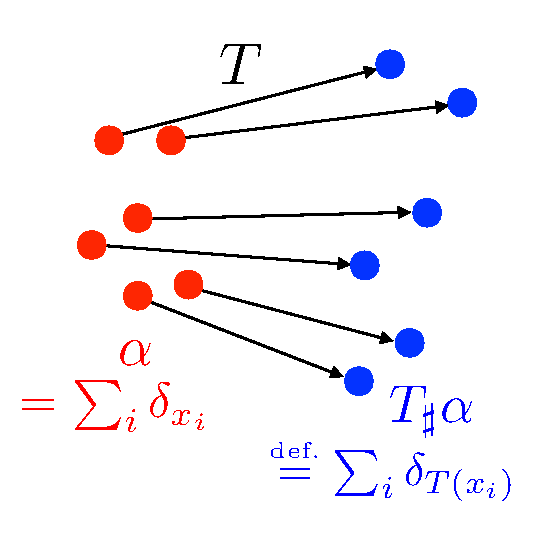
\includegraphics[width=.3\linewidth]{push-pull/push-forward}&
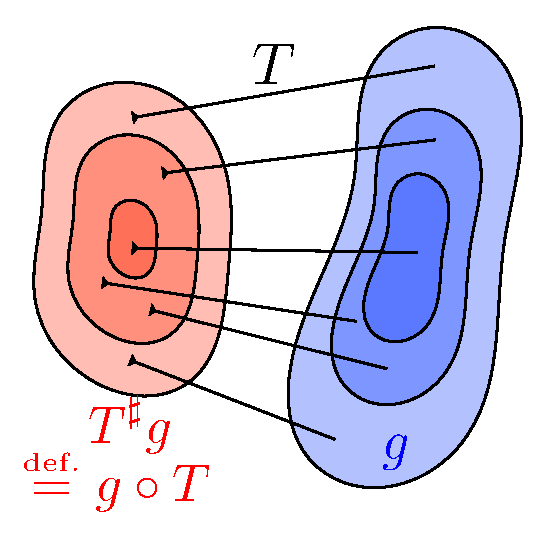
\includegraphics[width=.3\linewidth]{push-pull/pull-back}\\
Push-forward of measures & Pull-back of functions
\end{tabular}
\caption{\label{fig-push-pull}
Comparison of push-forward $\T_\sharp$ and pull-back $\T^\sharp$.
}
\end{figure}



A random variable $X$, equivalently, it is the push-forward of $\PP$ by $X$, $\al=X_\sharp\PP$.
%
Applying another push-forward $\be = \T_\sharp\al$ for $\T : \X \rightarrow \Y$, following~\eqref{eq-push-fwd}, is equivalent to defining another random variable $Y=\T(X) : \om \in \Om \rightarrow \T(X(\om)) \in Y$, so that $\be$ is the distribution of $Y$.
%
Drawing a random sample $y$ from $Y$ is thus simply achieved by computing $y=\T(x)$ where $x$ is drawn from $X$. 



%%%%%%%%%%%%%%%%%%%%%%%%%%%%%%%%%%%%%%%%%%%%%%%%%%%%%%%%%%%%%%%%%%%%%%%%%%%
\subsection{Brenier Theorem}


%%%%
\paragraph{Monge problem}

Monge problem~\eqref{eq-monge-discr} is extended to the setting of two arbitrary probability measures $(\al,\be)$ on two spaces $(\X,\Y)$ as finding a map $\T : \X \rightarrow \Y$ that minimizes
\eql{\label{eq-monge-continuous}
	\umin{\T} \enscond{ \int_{\X} \c(x,\T(x)) \d \al(x)  }{  \T_\sharp \al = \be }
}
The constraint $\T_\sharp \al = \be$ means that $\T$ pushes forward the mass of $\al$ to $\be$, and makes use of the push-forward operator~\eqref{eq-push-fwd}. 

For empirical measure with same number $n=m$ of points, one retrieves the optimal matching problem TODO explain.   
  


%%%%
\paragraph{Brenier's theorem}

The following celebrated theorem of~\cite{Brenier91} ensures that in $\RR^\dims$ for $p=2$, if at least one of the two inputs measures has a density, then Kantorovitch and Monge problems are equivalent.

\begin{thm}[Brenier]
	In the case $\X=\Y=\RR^\dims$ and $c(x,y)=\norm{x-y}^2$, if at least one of the two inputs measures (denoted $\al$) has a density $\density{\al}$ with respect to the Lebesgue measure, then the optimal $\pi$ in the Kantorovich formulation~\eqref{eq-mk-generic} is unique, and is supported on the graph $(x,\T(x))$ of a ``Monge map'' $\T : \RR^\dims \rightarrow \RR^\dims$. This means that $\pi = (\Id,\T)_{\sharp} \mu$, \emph{i.e.} 
\eql{\label{eq-brenier-map}
	\foralls h \in \Cc(\X \times \Y), \quad
		\int_{\X \times \Y} h(x,y) \d \pi(x,y) = \int_{\X} h(x,\T(x)) \d\mu(x).
}
Furthermore, this map $\T$ is uniquely defined as the gradient of a convex function $\phi$, $\T(x) = \nabla\phi(x)$, where $\phi$ is the unique (up to an additive constant) convex function such that $(\nabla\phi)_\sharp \mu=\nu$. This convex function is related to the dual potential $\f$ solving~\eqref{eq-dual-generic} as $\phi(x)=\frac{\norm{x}^2}{2}-\f(x)$.
\end{thm}


This results shows that in the setting of $\Wass_2$ with non-singular densities, the Monge problem~\eqref{eq-monge-continuous} and its Kantorovich relaxation~\eqref{eq-mk-generic} are equal (the relaxation is tight). This is the continuous analog of Proposition~\ref{prop-matching-kanto} for the assignment case~\eqref{prop-matching-kanto}, which states that the minimum of the optimal transport problem is achieved, when the marginals are equal and uniform, at a permutation matrix (a discrete map).
%
Brenier's theorem, stating that an optimal transport map must be the gradient of a convex function, should be examined under the light that a convex function is the natural generalization of the notion of increasing functions in dimension more than one. Optimal transport can thus plays an important role to define quantile functions in arbitrary dimensions, which in turn is useful for applications to quantile regression problems~\cite{carlier2016vector}.

Note also that this theorem can be extended in many directions. 
% 
The condition that $\al$ has a density can be weakened to the condition that it does not give mass to ``small sets'' having Hausdorff dimension smaller than $\dims-1$ (e.g. hypersurfaces). 
%
One can also consider costs of the form $\c(x,y)=h(x-y)$ where $h$ is a strictly convex function. 




- Brenier thm, need regularity of the *source*



\todo{Question of regularity of OT: need convexity of *target*}


%%%%%%%
\paragraph{Monge-Amp\`ere equation}

For measures with densities, using~\eqref{eq-pfwd-density}, one obtains that $\phi$ is the unique (up to the addition of a constant) convex function which solves the following Monge-Ampère-type equation
\eql{\label{eq-monge-ampere}
	\det(\partial^2\phi(x))  \density{\be}(\nabla\phi(x)) = \density{\al}(x)
}
where $\partial^2\phi(x) \in \RR^{\dims \times \dims}$ is the hessian of $\phi$. The Monge-Amp\`ere operator $\det(\partial^2\phi(x))$ can be understood as a non-linear degenerate Laplacian. In the limit of small displacements, $\phi=\Id + \epsilon\phi$, one indeed recovers the Laplacian $\Delta$ as a linearization since for smooth maps
\eq{
	\det(\partial^2\phi(x)) = 1 + \epsilon \Delta \phi(x) + o(\epsilon).
}
%
The convexity constraint forces $\det(\partial^2\phi(x)) \geq 0$ and is necessary for this equation to have a solution. 





%%%%%%%
\paragraph{OT in 1D}

For a measure $\al$ on $\RR$, we introduce the cumulative function
\eql{\label{eq-cumul-defn}
	\foralls x \in \RR, \quad \cumul{\al}(x) \eqdef \int_{-\infty}^x \d\al, 
}
which is a function $\cumul{\al} : \RR \rightarrow [0,1]$, and its pseudo-inverse  $\cumul{\al}^{-1} : [0,1] \rightarrow \RR \cup \{-\infty\}$ \eq{
	\foralls r \in [0,1], \quad \cumul{\al}^{-1}(r) = \umin{x} \enscond{x \in \RR \cup \{-\infty\} }{ \cumul{\al}(x) \geq r }.
}
%
That function is also called the generalized quantile function of $\alpha$. For any $p \geq 1$, one has
\eql{\label{eq-wass-cumul}
	\Wass_p(\al,\be)^p = \norm{ \cumul{\al}^{-1} - \cumul{\be}^{-1} }_{L^p([0,1])}^p = \int_0^1 | \cumul{\al}^{-1}(r) - \cumul{\be}^{-1}(r) |^p \d r.
}
This means that through the map $\al \mapsto \cumul{\al}^{-1}$, the Wasserstein distance is isometric to a linear space equipped with the $L^p$ norm, or, equivalently, that the Wasserstein distance for measures on the real line is a Hilbertian metric. 
This makes the geometry of 1-D optimal transport very simple, but also very different from its geometry in higher dimensions, which is not Hilbertian as discussed in Proposition~\ref{prop-negative-definite} and more generally in~\S\ref{sec-non-embeddability}.
%
For $p=1$, one even has the simpler formula
\begin{align}\label{eq-w1-1d}
	\Wass_1(\al,\be) &= \norm{ \cumul{\al} - \cumul{\be} }_{L^1(\RR)} = 
	\int_\RR | \cumul{\al}(x) - \cumul{\be}(x) | \d x \\
	&= \int_\RR \abs{ \int_{-\infty}^x \d(\al-\be) } \d x.
\end{align}
which shows that $\Wass_1$ is a norm (see~\S\ref{sec-w1-eucl} for the generalization to arbitrary dimensions). 
%
An optimal Monge map $\T$ such that $\T_\sharp \al=\be$ is then defined by
\eql{\label{eq-OT-map-1d}
 	\T = \cumul{\be}^{-1} \circ \cumul{\al}.
}
Figure~\ref{fig-1d-ot} illustrates the computation of 1-D OT through cumulative functions. It also displays displacement interpolations, computed as detailed in~\eqref{eq-displacement-1d-cumul}, see also Remark~\ref{rem-bary-1d}. For a detailed survey of the properties of optimal transport in 1-D, we refer the reader to~\cite[Chapter 2]{SantambrogioBook}.



\newcommand{\MyFigCumulMeas}[1]{\includegraphics[width=.28\linewidth]{1d-cumulative/#1}}
\newcommand{\MyFigCumulCum}[1]{\includegraphics[width=.2\linewidth]{1d-cumulative/#1}}
\begin{figure}
\centering
\begin{tabular}{@{}c@{\hspace{1mm}}c@{\hspace{1mm}}c@{}}
\MyFigCumulMeas{input-mu}&
\MyFigCumulMeas{input-nu}&
\MyFigCumulMeas{interp-bary}\\
$\mu$ & $\nu$ & ${ (t\T+(1-t)\Id)_\sharp \mu}$
\end{tabular}
%%%%
\begin{tabular}{@{}c@{\hspace{2mm}}c@{\hspace{2mm}}c@{\hspace{2mm}}c@{}}
\MyFigCumulCum{cumul}&
\MyFigCumulCum{icumul}&
\MyFigCumulCum{transports}&
\MyFigCumulCum{interp-cumul}\\
$(\cumul{\al},\cumul{\be})$ & 
$(\cumul{\al}^{-1},\cumul{\be}^{-1})$ & 
$(T,T^{-1})$ &
$(1-t)\cumul{\al}^{-1}+t\cumul{\be}^{-1}$ 
\end{tabular}
\caption{\label{fig-1d-ot}
Computation of OT and displacement interpolation between two 1-D measures, using cumulant function as detailed in~\eqref{eq-OT-map-1d}. 
}
\end{figure}




%%%%%%%
\paragraph{OT on Gaussians}

\todo{First in 1D}

If $\al = \Nn(\mean_\al,\cov_\al)$ and $\be = \Nn(\mean_\be,\cov_\be)$ are two Gaussians in $\RR^\dims$, then one can show that the following map
\eql{\label{eq-transport-Bures}T:x\mapsto \mean_\be + A(x-\mean_\al),}
where 
$$A=\cov_\al^{-\tfrac{1}{2}}\Big(\cov_\al^{\tfrac{1}{2}}\cov_\be\cov_\al^{\tfrac{1}{2}}\Big)^{\tfrac{1}{2}}\cov_\al^{-\tfrac{1}{2}}=\transp{A},$$
is such that $T_\sharp \rho_\al = \rho_\be$. Indeed, one simply has to notice that the change of variables formula~\eqref{eq-pfwd-density} is satisfied since
$$
\begin{aligned}\rho_\be(T(x))&=\det(2\pi\cov_\be)^{-\tfrac{1}{2}} \exp(-\dotp{T(x)-\mean_\be}{\cov_\be^{-1}(T(x)-\mean_\be)})\\
&= \det(2\pi\cov_\be)^{-\tfrac{1}{2}} \exp(-\dotp{ x-\mean_\al}{\transp{A}\cov_\be^{-1}A(x-\mean_\al)}) \\
&= \det(2\pi\cov_\be)^{-\tfrac{1}{2}} \exp(-\dotp{ x-\mean_\al}{\cov_\al^{-1}(x-\mean_\al)}),
\end{aligned}$$
and since $T$ is a linear map we have that 
$$|\det T'(x)|= \det A = \left(\frac{\det\cov_\be}{\det\cov_\al}\right)^{\tfrac{1}{2}}$$
 and we therefore recover $\rho_\al=|\det T'| \rho_\be$ meaning $T_\sharp \al = \be$. Notice now that $T$ is the gradient of the convex function $\psi:x\mapsto \tfrac{1}{2}\dotp{x-\mean_\al}{A (x-\mean_\al)} + \dotp{\mean_\be}{x}$ to conclude, using Brenier's theorem~\cite{Brenier91} (see Remark~\ref{rem-exist-mongemap}) that $T$ is optimal. Both that map $T$ and the corresponding potential $\psi$ are illustrated in Figures~\ref{fig-gaussians-2d-T} and~\ref{fig-gaussians-2d-psi}
 
 
With additional calculations involving first and second order moments of $\rho_\al$, we obtain that the transport cost of that map is
\eql{\label{eq-dist-gauss}
	\Wass_2^2( \al,\be ) = \norm{ \mean_\al - \mean_\be }^2 + \Bb(\cov_\al,\cov_\be)^2
}
where $\Bb$ is the so-called Bures' metric~\cite{bures1969extension} between positive definite matrices (see also~\cite{,forrester2016relating}),
\eql{\label{eq-bure-defn}
	\Bb(\cov_\al,\cov_\be)^2 \eqdef \tr\pa{
		\cov_\al + \cov_\be - 2 ( \cov_\al^{1/2} \cov_\be \cov_\al^{1/2} )^{1/2}
	},
}
where $\cov^{1/2}$ is the matrix square root. One can show that $\Bb$ is a distance on covariance matrices, and that $\Bb^2$ is convex with respect to both its arguments. 
In the case where $\cov_\al = \diag(r_i)_i$ and $\cov_\be = \diag(s_i)_i$ are diagonals, the Bures metric is the Hellinger distance
\eq{
	\Bb(\cov_\al,\cov_\be) = \norm{ \sqrt{r}-\sqrt{s} }_2.
}
For 1-D Gaussians, $\Wass_2$ is thus the Euclidean distance on the 2-D plane $(\mean,\sqrt{\cov})$, as illustrated in Figure~\ref{fig-1d-gaussian}. 
%
For a detailed treatment of the Wasserstein geometry of Gaussian distributions, we refer to~\cite{takatsu2011wasserstein}.





\begin{figure}
\centering
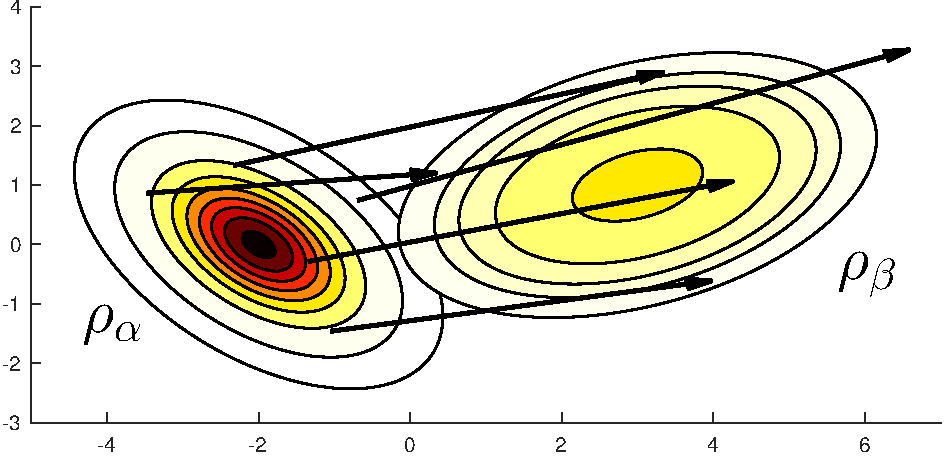
\includegraphics[width=.4\linewidth]{gaussians-2d/gaussians1.pdf}
\caption{\label{fig-gaussians-2d-T} Two Gaussians $\rho_\al$ and $\rho_\be$, represented using the contour plots of their densities, with respective mean and variance matrices $\mean_\al=(-2,0),\cov_\al=\frac{1}{2}\left(1 -\tfrac{1}{2};-\tfrac{1}{2}  1\right)$ and $\mean_\be=(3,1), \cov_\be=\left(2, \tfrac{1}{2}; \tfrac{1}{2}, 1\right)$. The arrows originate at random points $x$ taken on the plane and end at the corresponding mappings of those points $T(x)=\mean_\be + A(x-\mean_\al)$.}
\end{figure}



\begin{figure}
\centering
\begin{tabular}{@{}c@{\hspace{15mm}}c@{}}
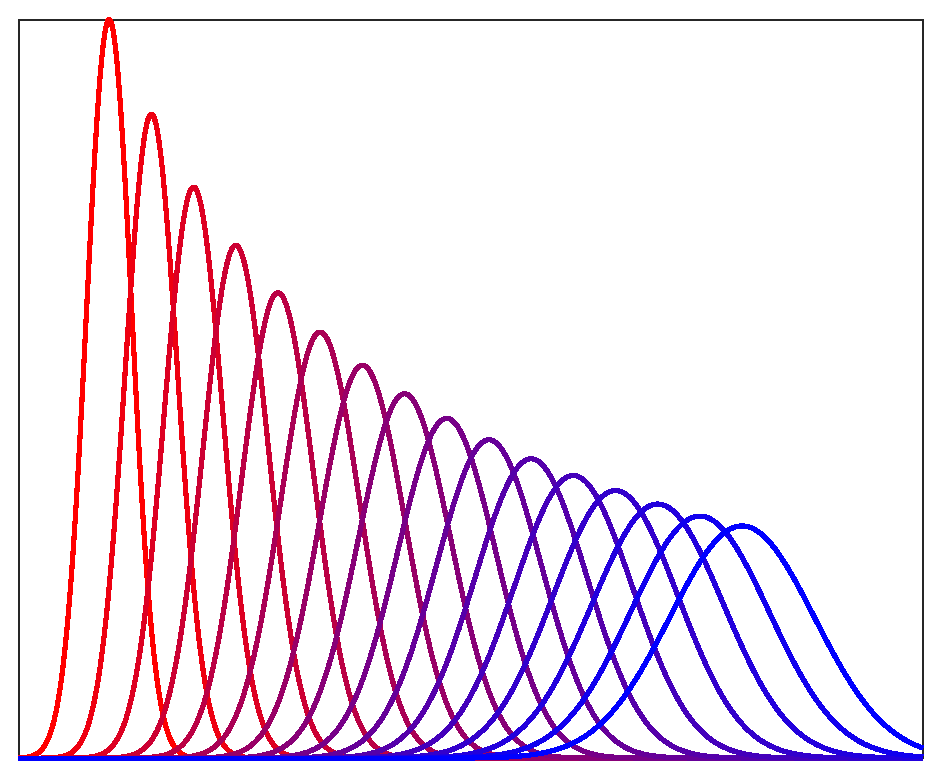
\includegraphics[width=.25\linewidth]{gaussian-1d/interp-density}&
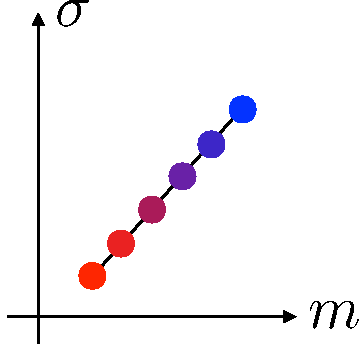
\includegraphics[width=.2\linewidth]{gaussian-1d/gaussian-param}
\end{tabular}
\caption{\label{fig-1d-gaussian}
Computation of displacement interpolation between two 1-D Gaussians. 
%
Denoting $\Gg_{m,\si}(x) \eqdef \frac{1}{\sqrt{2\pi}s}e^{-\frac{(x-m)^2}{2s^2}}$ the Gaussian density, it thus shows 
the interpolation $\Gg_{(1-t)m_0+t m_1,(1-t)\si_0+t \si_1}$.
}
\end{figure}





